% Rien d'autre à faire qu'afficher le titre
\begin{frame}
\titlepage 
\end{frame}

\begin{frame}
    \frametitle{Clarification sur le sujet}
    \begin{figure}
        \centering
        \begin{minipage}{.5\textwidth}
            \centering
            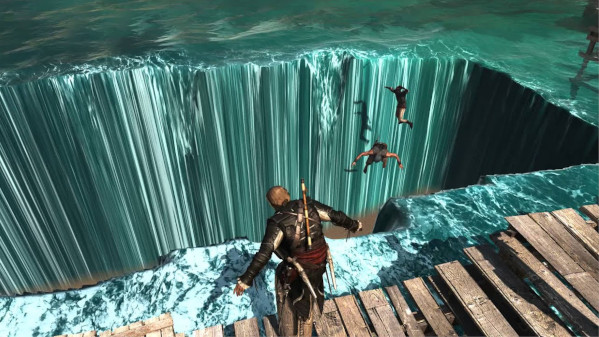
\includegraphics{figures/black_flag_not_water_simulation.jpg}
            \captionof{figure}{Assassin's Creed: Black Flag - Pas de simulation de fluide}
            \label{fig:test1}
        \end{minipage}%
        \begin{minipage}{.5\textwidth}
            \centering
            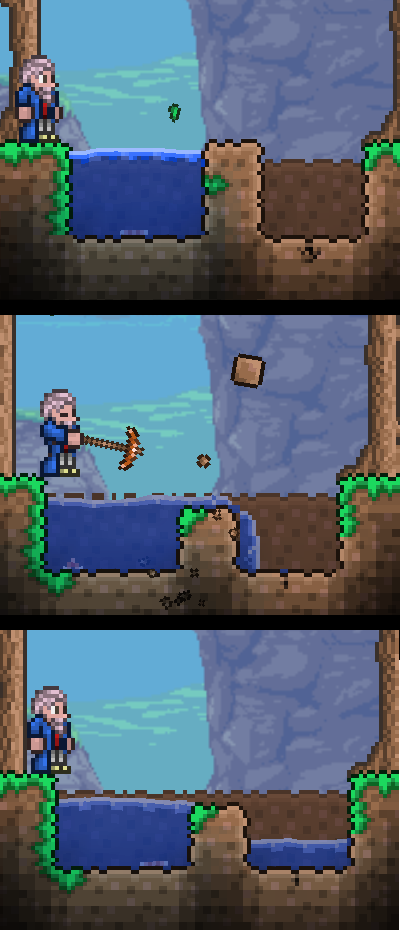
\includegraphics[height=6cm]{figures/terrarria_fluid_sim.png}
            \captionof{figure}{Terrarria - Simulation de fluide}
            \label{fig:test2}
        \end{minipage}
    \end{figure}
\end{frame}

% La table des matières utilise ce que vous donnez aux commandes \section et 
% \subsection tout au long de la présentation.
\begin{frame}
\frametitle{Plan de l'exposé} 
\tableofcontents 
\end{frame}
